\documentclass{ws-jai}
% This is a sample LaTeX input file.
\usepackage[latin9]{inputenc}
\usepackage{graphicx}
%\usepackage[dvipdfmx]{graphicx}
\DeclareGraphicsExtensions{.eps,.png,.pdf,.jop}
\DeclareGraphicsRule{.png}{eps}{.bb}{}

\usepackage[breaklinks,colorlinks,urlcolor=blue,citecolor=blue,linkcolor=blue]{hyperref}
\usepackage{url}

%\usepackage[authoryear]{natbib}
\usepackage{subfigure}
\usepackage{color}
\usepackage{threeparttable}
  



\begin{document}

%\catchline{}{}{}{}{} % Publisher's Area please ignore

\markboth{C.~H.~ Niu et. al.}{2D-FFT Method}

\title{Correlator built on Roach2-GPU framework for Tianlai Array\footnote{This paper is found by  China Scholarship Council }}  

\author{
%C.~H.~Niu$^{1,2,3}$, Q.~X.~Wang$^{2,4}$, D.~ Macmahon$^3$, J.~X.~Li$^2$,  F.~Q.~Wu$^{2\dagger}$,G.~Shippee$^3$, H.~J.~Tian$^4$, X.~L.~Chen$^2$, D.~Werthimer$^3$
}

\address{
\small
$^1$Central China Normal University ,Luoyu Road, Wuhan, China\\
$^2$National Astronomy Observatory , Chinese Academy of Sciences \\Datun(A) Road, No.30,Beijing, China\\
$^3$University of California Berkeley, Campbell Hall 339, Berkeley CA 94720\\
$^4$China Three Gorges University,Yichang China 443002
}

\maketitle
\corres{$^\dagger$Corresponding author:F.~Q.~Wu. Email: \url{wufq@bao.ac.cn}}

% UNCOMMENT THE LINES BELOW IF YOU WISH TO USE BIBTEX
%Citations may be made using the natbib commands \citet{},\citep{} etc.
%%\usepackage[authoryear]{natbib}
%\bibpunct{(}{)}{;}{a}{}{,}
%\setlength{\bibsep}{0.3mm}

%f
\begin{abstract}
Correlators play an important role in radio astronomy interferometery. Considering Field Programmable Gate Arrays (FPGA) and Application Specific Integrated Circuit technologies require longer development periods, we decided to build a correlator based on the ROACH2-GPU framework, as it is more scalable, more flexible, and quicker to deploy. Our correlator includes an F-engine used for Analog to Digital Conversion (ADC) and Polyphase Filter Bank (PFB) computation, built on a ROACH2 board\footnote{ \url{https://casper.berkeley.edu/wiki/ROACH2}}(Reconfigurable Open Architecture Computing Hardware); and an X-engine focused mainly on conjugate multiply-accumulate operation (CMAC), built on GPUs (Graphical Processing Units). The correlator is designed for the Tianlai Interferometer Array.

\end{abstract}
%
\keywords{
Correlator, Tianlai array, ROACH2, GPU
}

\section{Introduction}

	In radio astronomy, correlators are implemented with the purpose of increasing visibility through the process of correlation. With this visibility information, one can reconstruct the sky map\cite{1986isra.book.....T}. The process of correlation, which involves two or more signals, can be performed in two ways. In XF type correlation, the signal is first convolved and then a Fourier Transform is taken. In FX type correlation, the Fourier Transform is taken first and then the signals are cross multiplied. As multiplying in frequency domain is equivalent to convolving in the time domain, the results from these two types of correlators are identical. With larger telescope arrays, FX correlation is much quicker than XF correlation\cite{2016JAI.....502002P}, thus FX correlation is more proper to use in a large array system.
	 
	Tianlai is a radio interferometer array located in Hongliuxia, Xinjiang, in the north-west of China\cite{2012IJMPS..12..256C}. It is designed for BAO(?) through observing the 21cm line. The array includes three cylinder reflectors and 16 dish telescopes. Each cylinder is 40m long with 15m wide, and each dish telescope has a 6-meter aperture. The Tianlai Array is shown in Figure \ref{fig:Tianlai}. Inputs for the Tialai pathfinder experiment are: the cylinder array, with $96\times2=192$ inputs; and the dish array, with $16\times2=32$ inputs. The number of inpus will increase in the future, which will cause computation to become even more costly for correlator. \textbf{By the demand of Tianlai, we plan to build a correlator based on the ROACH2-GPU framework. Processes like ADC, FFT called F-engine are implemented on ROACH2 Board, Cross Multiply Accumulation  which is simple in computational complexity but with high computational intensity accomplished in GPU, we called that part X-engine. Data transfer between ROACH2 and GPU server via 10Gbit/s switch.} isn't this already mentioned in the previous paragraph?

	This correlator has already been partially installed and tested in the Hongliuxia observatory. In this paper we introduce the sketch of the correlator in Section \ref{sec:1}; the F-engine in Section \ref{sec:F-engine}; the X-engine in Section \ref{sec:X-engine}; the network system in Section \ref{sec:Local Network}; some checks and experiments for the correlator in Section \ref{sec:experiment}; and a summary of the work with future prospects in Section \ref{sec:summary}.

\begin{figure}[t]
 \centering
 %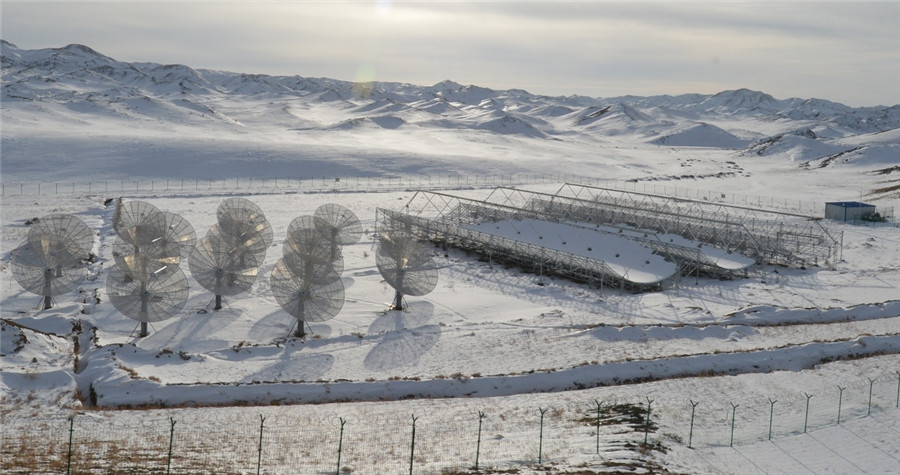
\includegraphics[width=0.9\textwidth]{./picture/Tianlai.jpg}
 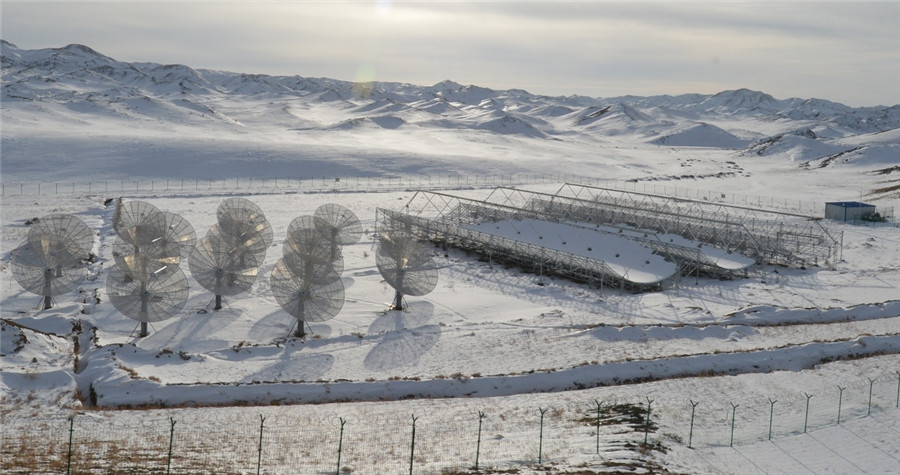
\includegraphics[width=0.9\textwidth]{./picture/Tianlai.jpg}
\caption{Tianlai interferometer Array. On the left is the 16 dish telescope. On the right are the three cylinder telescopes.\label{fig:Tianlai}}
\end{figure}

\section{Whole System}\label{sec:1}
  

	The ROACH2-GPU framework for correlators is popular in many radio interferometer arrays, including PAPER (Precision Array for Probing the Epoch of Re-ionization)\cite{2010AJ....139.1468P}, LEDA (Large Aperture Experiment to Detect the Dark Ages), and others. Our structure builds from the PAPER correlator model \cite{2008PASP..120.1207P}, and creates a flexible and scalable hybrid correlator system for the Tianlai project.
	
	 For the whole correlator system, we assume the F-engine has $M$ ROACH2 nodes, and the X-engine has $N$ GPU nodes.  Every ROACH2 node handles $m$-way analog radio inputs, and after performing a FFT, outputs $m$ spectrums. Additionally, each spectrum has $F$ frequency points. To optimize data traffic, each GPU node processes ${F}/{N}$ frequency points, and each frequency point includes $M\times m$ conjugate multiply computations. Therefore the ROACH node should divide the $F$ point spectrum into $N$ bands, and then send the specified band to the corresponding GPU node. We will present the F-engine model in detail in \ref{sec:F-engine}. In the GPU node, the ${F}/{N}$ frequency points will be distributed to $N$ cores to do conjugate multipliclation accumulation. We will introduce the X-engine in detail at \ref{sec:X-engine}.            
	  
	The structure for the Tianlai correlator is shown in Figure \ref{fig:structure}. The ROACH node can be controlled by a ROACH2-server through the Internet. Via a KATCP (Karoo Array Telescope Control Protocol) protocol, one can load the specified FPGA model to the ROACH2 board. We designed several FPGA models on the CASPER (Collaboration for Astronomy Signal Processing and Electronics Research) platform, such as an ADC raw data sample model which outputs the digital data by sampling the analog signal directly, \textbf{(32-input and 64-input model which are for the test of small scalar experiment based on PAPER model.)}?  We also built two different FFT length (1024 and 512) correlator models for the different frequency resolution requirements of Tianlai. The six ROACH2 boards which are referred to as F-engines, sample 192-input analog signals from the receiver with 8 bit resolution. The sampled data goes through an FFT, Equalizer, Transpose, and 10Gb Ethernet functional block, ultimatley reaching the 10Gb Ethernet switch. Each ROACH2 board has 4 10Gb Ethernet ports connected to a switch, and we assign static MAC addresses to each port on the switch. In addition, we divide the network into several sub-network VLANs. In the X-engine, we implement a distributed computational structure to do the CMAC. We have 8 GPU nodes to deal with different frequency bands, and in each GPU node, we installed two GTX690 GPUs, each equipped with two GPU cores. Thus each GPU node can compute the conjugate multiply accumulation for 128 frequency points from 192 inputs. Hashpipe is used to manage thread and data transfer in each GPU node. 
		
	The required number of ROACH2 boards is dependent on the number of antenna inputs. We have 2 ADC daughter boards installed in every ROACH2 board, while each ADC has 16 inputs. If we only consider the cylinder telescopes, we have 192 inputs, so 6 ROACH2 boards are needed. The number of GPU nodes is determined by the computational intensity. After several tests, we found the peak computational performance for each GPU core is 1.2 TFLOPS, giving us a total of 4.8 TFLOPS peak computational performance for each GPU node with 4 cores. The total computational intensity for Tianlai pathfinder experiment is thus 35.6 TFLOPS. Therefore we presume 8 GPU nodes will meet the demand for the present system.
\begin{figure}[t]
 \centering
 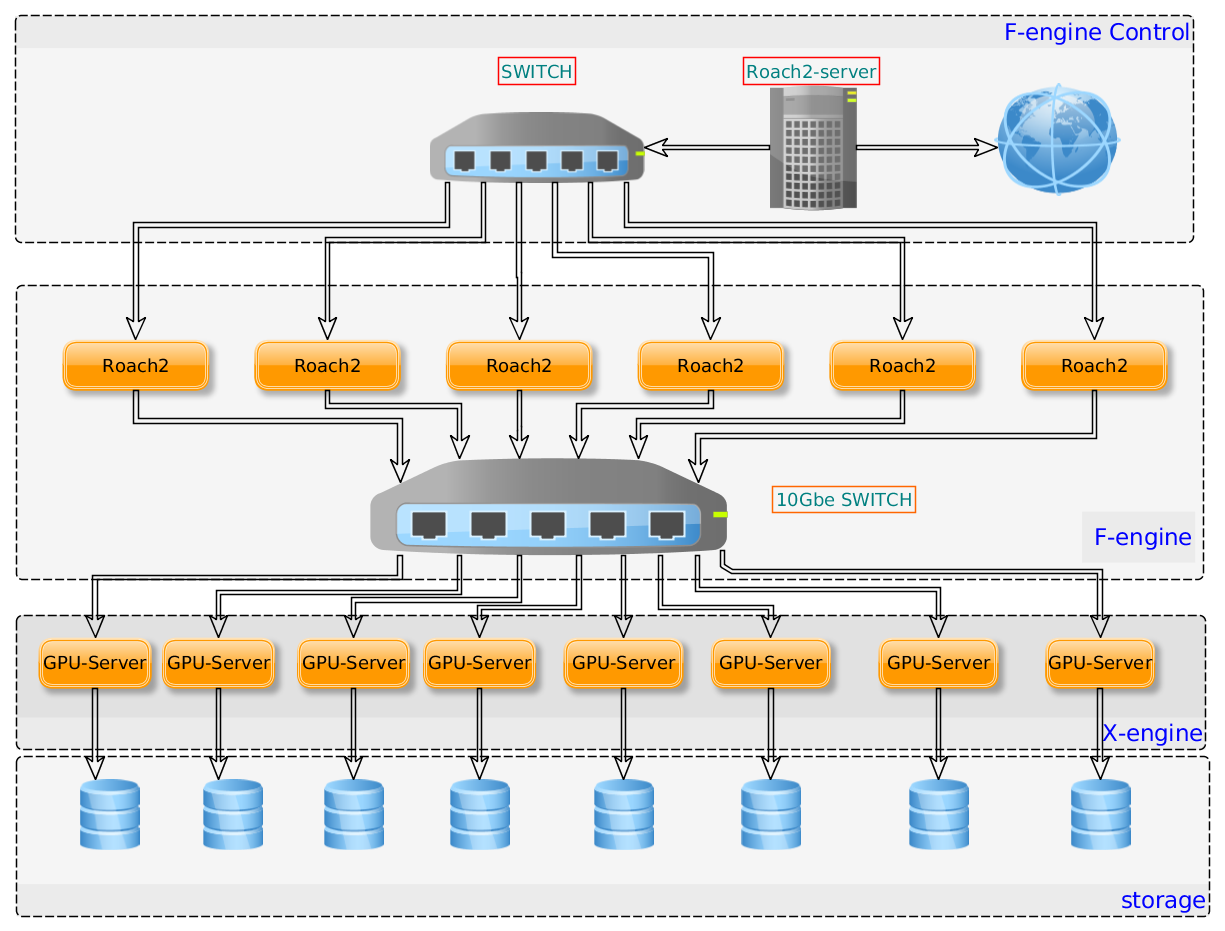
\includegraphics[width=0.9\textwidth]{./picture/structure1.eps}
\caption{Structure of Tianlai Correlator.\label{fig:structure}}
\end{figure}
\\
\subsection{F-engine}\label{sec:F-engine}
	The F-engine model is built on the CASPER platform. This platform allows the user to focus on the design and function of the model by introducing a graphical user interface which abstracts away from FPGA code. Most ROACH2 hardware already has its corresponding GUI yellow block implemented by CASPER developers\footnote{\url{https://casper.berkeley.edu/}}. In our correlator, the F-engine is expected to have the ability of ADC, FFT, frequency dependent data bit choosing, and the sending of different frequency bands of data from all antenna inputs to the corresponding GPU nodes. We can realize these functions by dragging the corresponding blocks from the CAPSER tools and considering the data interface, delay and data flow issue.

\subsubsection{Function Blocks\label{sec:function model}}
	The demand of the Tianlai correlator is similar to that of the PAPER correlator. As a result, our F-engine model is based on the PAPER F-engine model that is designed by David Macmahon \citep{paper_correlator}. The F-engine sketch is showed in Figure \ref{fig:f-engine}. As a radio-frequency interface, 2 16-input ADC daughter boards are mounted on a ROACH2 board. Each input is sampled with 8-bit resolution and then transferred to a PFB block, where the FFT is processed using a polyphase filter minimize energy leakage. 
	
\begin{figure}[t]
 \centering
 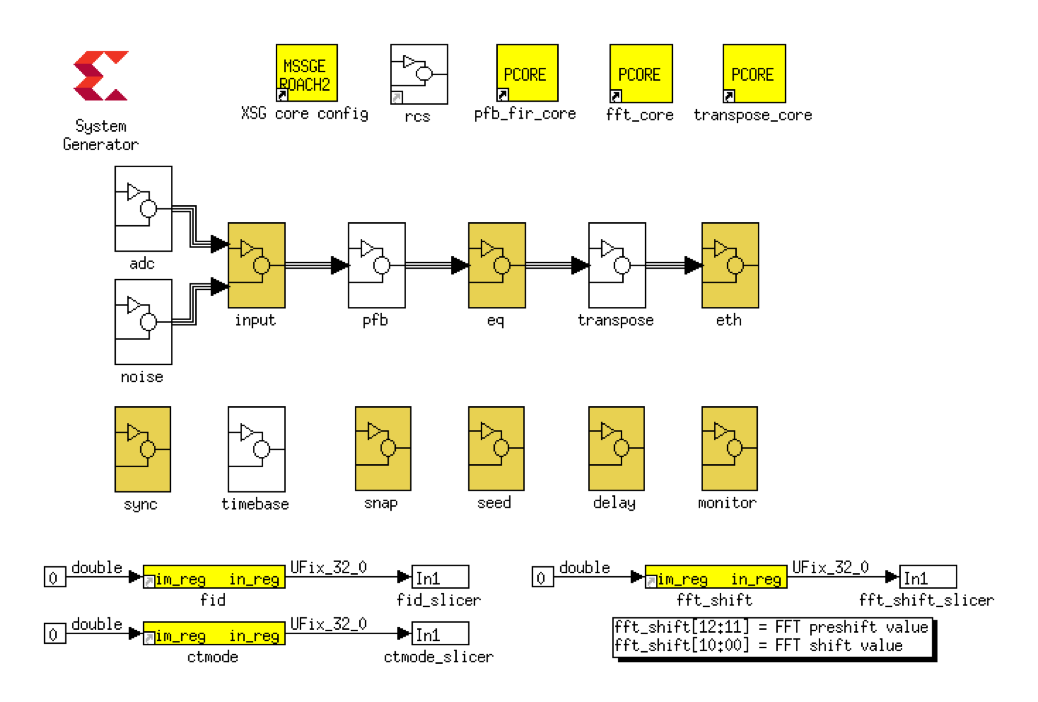
\includegraphics[width=0.9\textwidth]{./picture/f-engine1.eps}
\caption{F-engine model modified from PAPER correlator\label{fig:f-engine}}
\end{figure}


	To reduce the data exchange amount in the switch, we divide the 18-bit data into 4 bits chunks before sending it to the Ethernet.  Because different receivers have different frequency responses, we use an Equalizer block to take the data bits at the correct position corresponding to the correct frequency channels. Each frequency channel of each input will have its own adjustment factor. After the Equalizer block, data flow for each input is divided into a 4-bit real and a 4-bit imaginary component. 

\subsubsection{Transpose\label{sec:Transpose}}	
\begin{figure}[t]
 \centering
 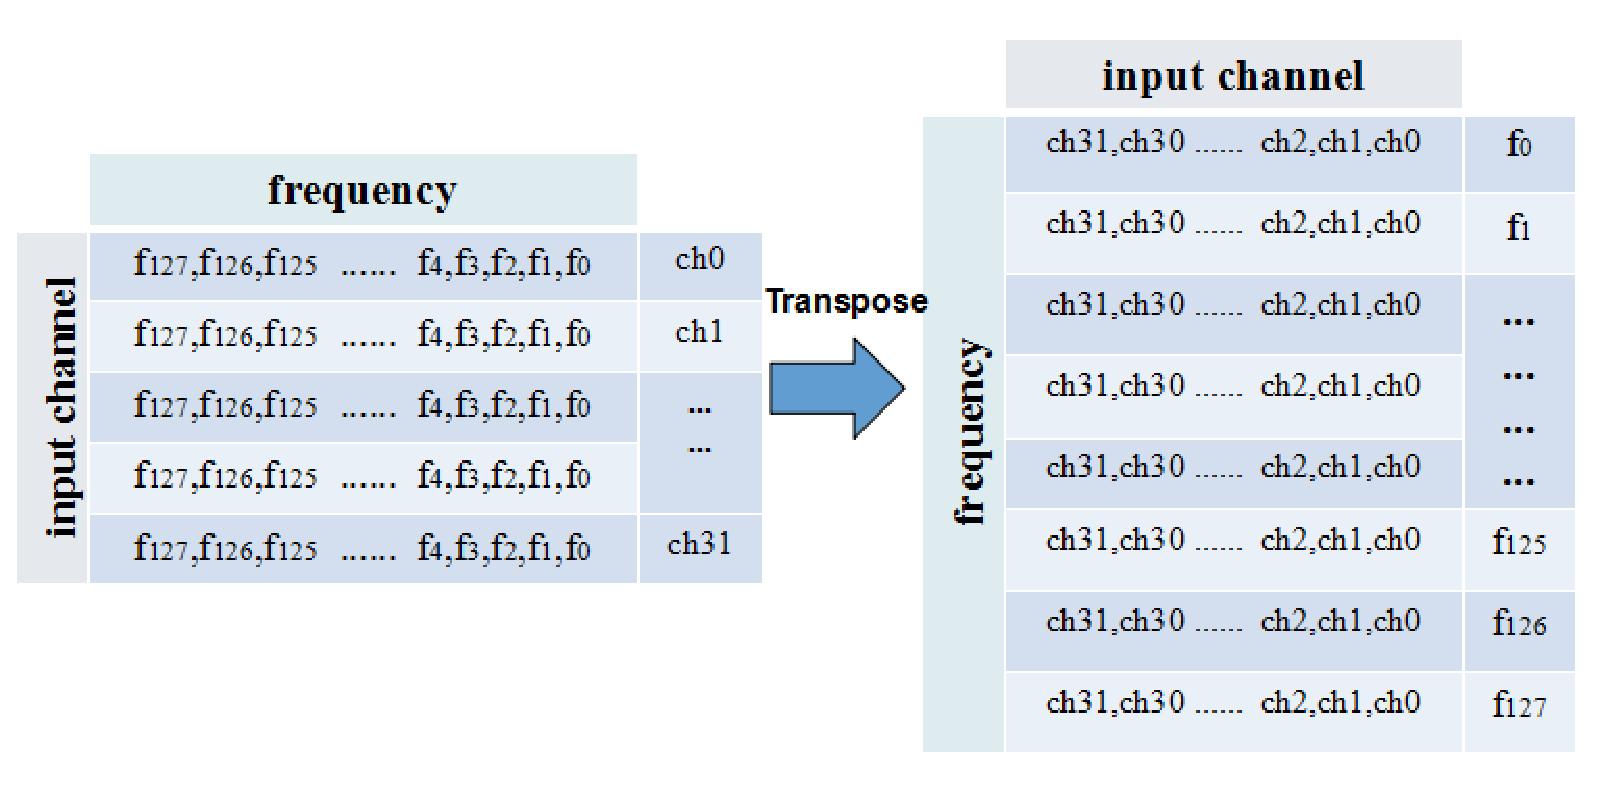
\includegraphics[width=0.9\textwidth]{./picture/transpose.eps}
\caption{Dataflow conversion of the Transpose. Left: Original data flow. Right: Transposed data flow.\label{fig:transepose}}
\end{figure}


   For the digital data after the ADC and FFT, various frequency data of a particular signal channel and time  is arranged in a successive order in the data flow. However, frequency channels must be distributed among a number of servers simultaneously, so suffering and making a transposition are mandatory before sending X engine with the frequency band data from all signal channels for a particalar time.  
	%As introduced in last section, different GPU node will process different part of frequency band from all antennas.  Before 
        %The different band are decided by F-engine Ethernet. but it also need to recognize that band is from which antenna input so that they could do conjugate multiply between inputs.
	%Voltage data go through FFT will become frequency points data flow, but each GPU node process one frequency band for all antenna inputs. 
        This need convert data shape from $[inputs,frequency]$ to $[frequency,inputs]$, like figure \ref{fig:transepose} shows. This operation could be achieved in a dual-port RAM through writing, reading from different address,\textcolor{red}{ alternative destination IP and changing header}.  Figure \ref{fig:transepose2} shows the overview of block design, if one output reading and writing address of dual-port RAM, we could see how exactly the reading and writing address change under flag signal from '$tid$','$fid$' etc.

\begin{figure}[t]
 \centering
 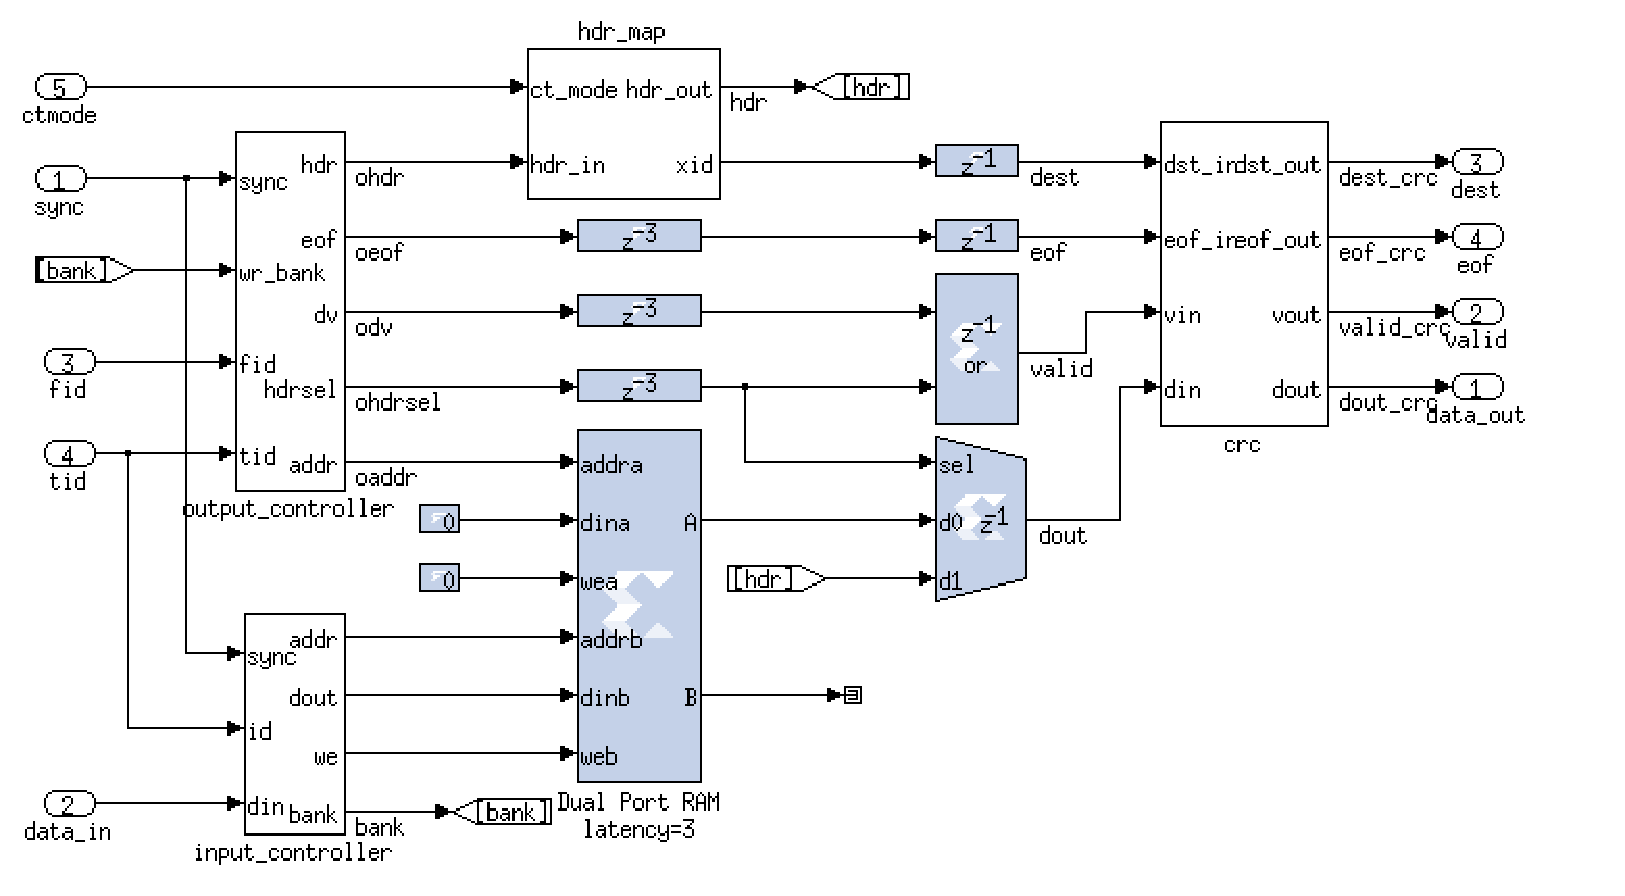
\includegraphics[width=0.9\textwidth]{./picture/transpose2.eps}
\caption{Structure of the second class sub-module in Transpose. One can modify the dest IP and packet size in this model.\label{fig:transepose2}}
\end{figure}

%\begin{figure}
%\epsscale{1}
%\plotone{address1.png}
%\epsscale{1}
%\plotone{address2.png}
%\caption{The output of Writing and Reading address of Dual port RAM. Writing address varied with clock (uppder); Reading address varied with clock(bottom). \label{fig:address}}
%\end{figure}

The ethernet block is the last block of the F-engine model. The only difference between the models used on the ROACH2 nodes is the IP and MAC configurations for the Ethernet block. One ROACH2 node has four 10Gbps ports. Without using the loopback mode used in the PAPER model, all of the Ethernet ports only send and do not receive packets, and each of them will have a different IP \textcolor{red}{information} decided by '$tid$'. Detailed strategy for IP assignment is described in sec \ref{sec:IP assignment}
	
When the F-engine is implemented, one can simulate the design on Matlab with CASPER tools. After \textcolor{red}{de-bugging} the model from the simulation, a 'bof' file is generated which can be uploaded to the FPGA as firmware.
  
\subsubsection{Control System}

	Each ROACH2 node is installed with a Power PC that runs a linux system. The ROACH2 server has a service called Network File System (NFS), which allows for the sharing of files, such as 'bof' files, with the Power PC on the ROACH2 node. Any time the ROACH2 boots up, it will load the linux kernel from the ROACH2 server or from the on-board memory chip. These booting methods are referred to as 'Net boot' or 'Solo boot', respectively. When the whole system is running under Net boot, all ROACH2 boards load the 'bof' files from the NFS on ROACH2 server. 
	
        There are sync ports in all functional blocks of a single ROACH2 node. The sync port ensures every component inside the model is \textcolor{red}{ready to run}. However, the clocks are not synchronous between different ROACH2 nodes. In this F-engine model, a sync model is used to synchronize all ROACH2 nodes to the same clock cycle by sending a 1PPS signal to each node. After all the parameters, such as the IP and MAC addressess are set, a sync signal called the 'Arm signal' is sent to each node. Then, all the ROACH2 nodes wait for a 1PPS signal to trigger the system. Arm signals at the different nodes are not required to be synchronized, but the 1PPS signals are made simultaneous by choosing the same length of cable for each signal. After this operation, all the ROACH2 nodes will be synchronized. A diagram is showed in Figure \ref{fig:1pps}.
\begin{figure}[t]
 \centering
 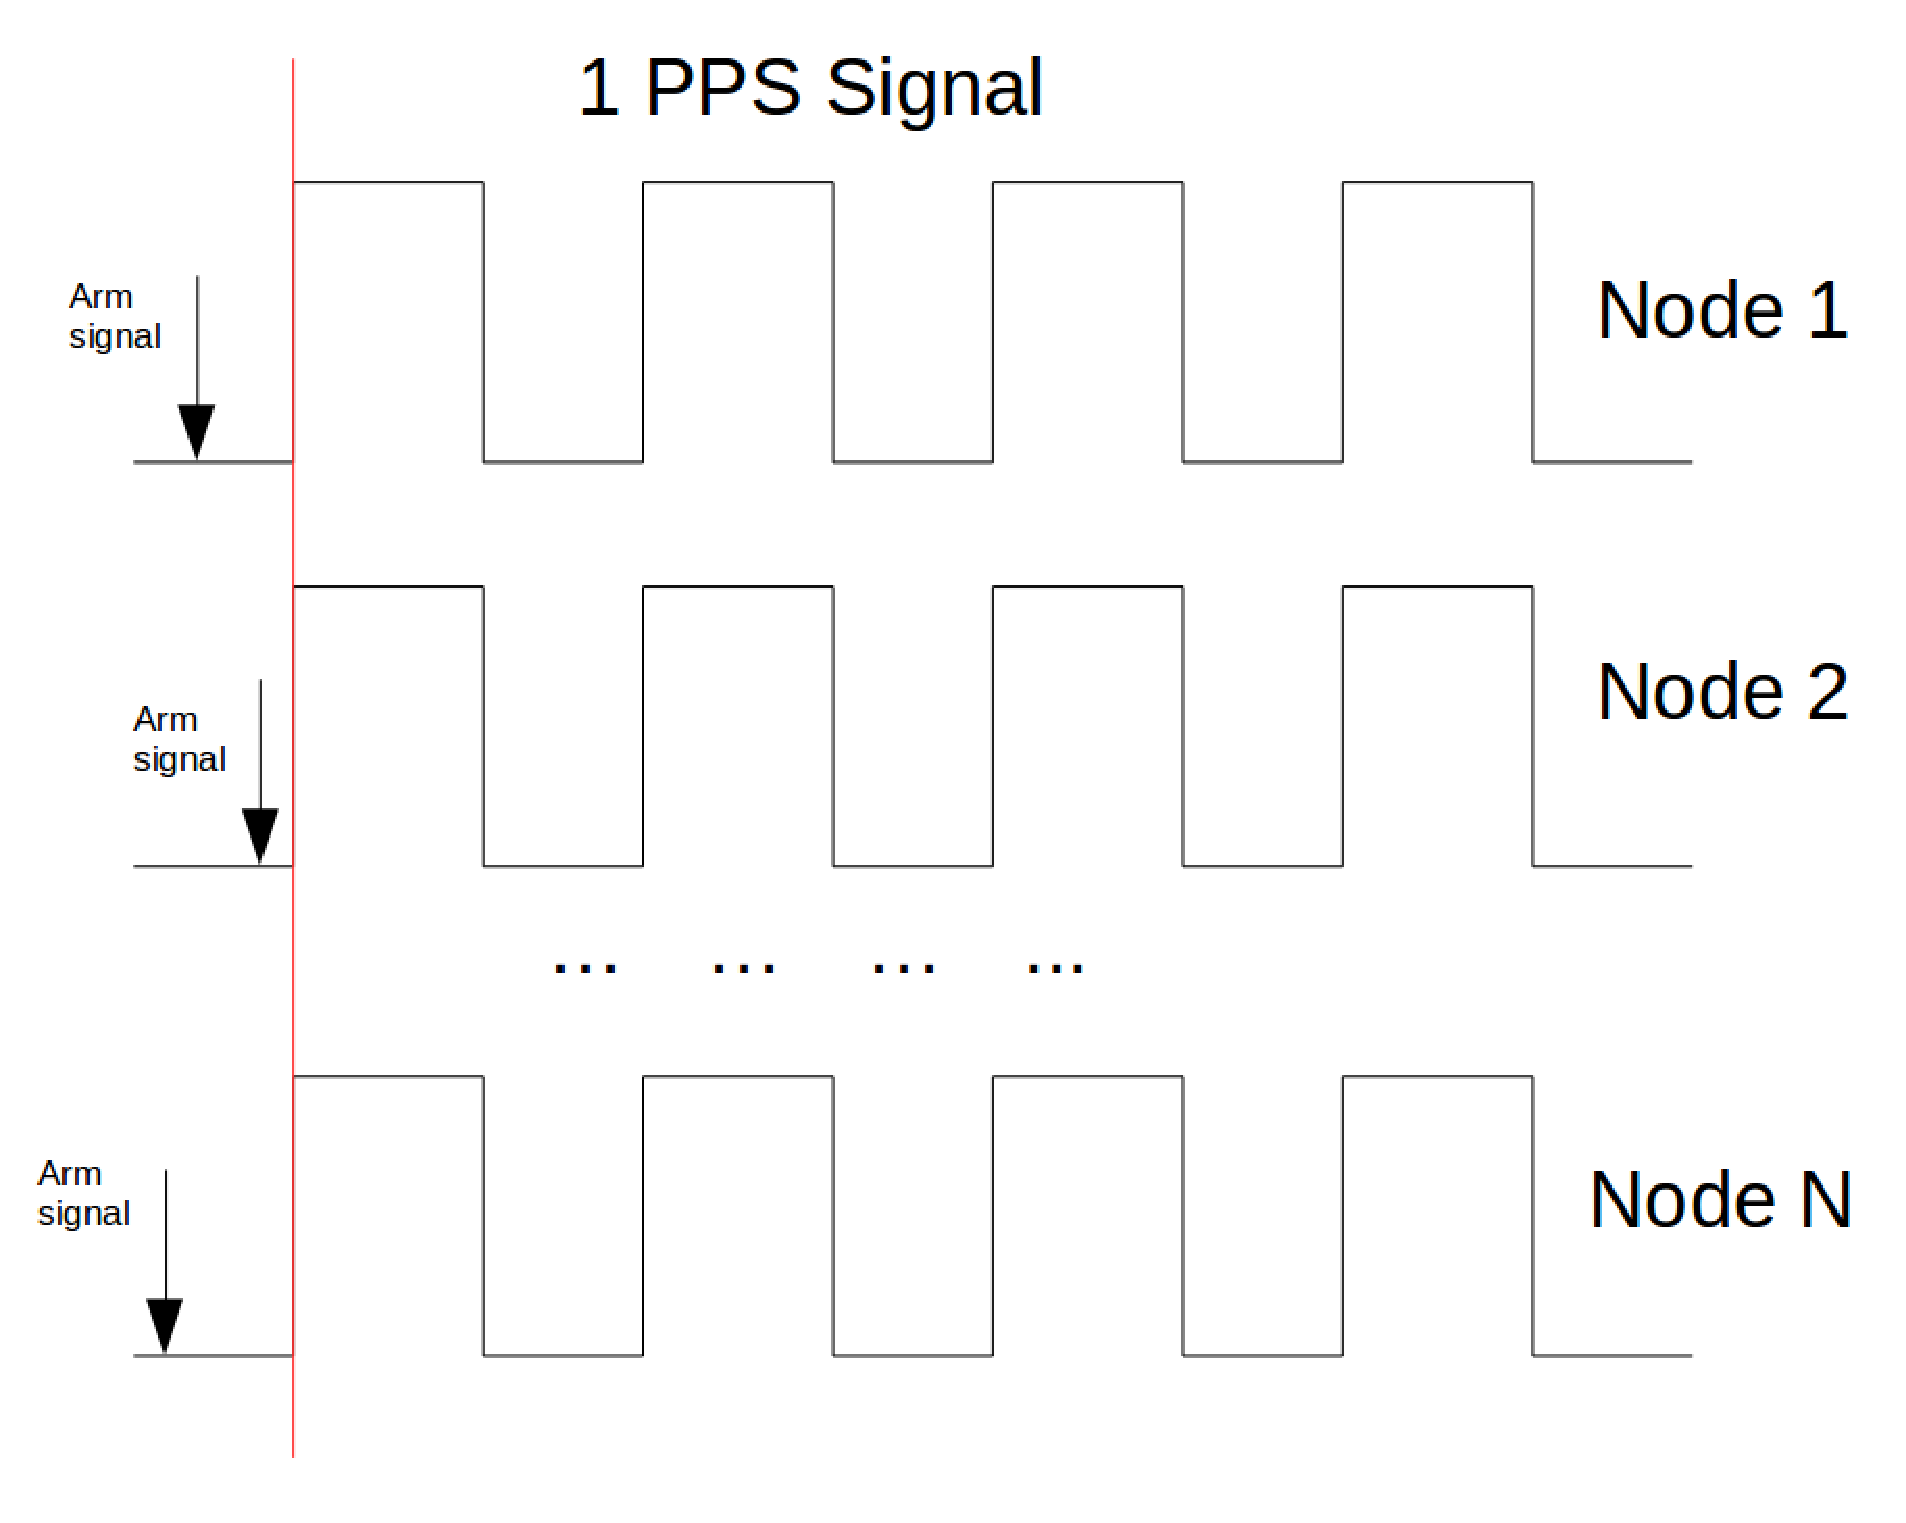
\includegraphics[width=0.5\textwidth]{./picture/1pps_sync.eps}
\caption{Synchronizing N ROACH2 nodes. The red lines indicate the start trigger using 1PPS signal\label{fig:1pps}}
\end{figure}


\subsection{X-engine}\label{sec:X-engine}

The X-engine in this system is mainly responsible for packet receiving, data distribution, Conjugate Multiply Accumulation and data storage. For one GPU node, there are 2 GTX690 cards, each containing 2 GPU cores, 2 CPUs and four 10 Gbits NICs. These four GPU cores work separately, each processing the CMAC of 32 frequency points. The CMAC process uses the 'xGPU' package provided by Michael Clark etc. \cite{2013IJHPC..27..178C}. The 'xGPU' code is written in CUDA-C and is optimized on GPU memory resources by specific thread tasks. It was originally designed to solve large array signal correlation processes.

\subsubsection{Thread Manager:Hashpipe}	
	
	Data management in each GPU node is done via Hashpipe\footnote{\url{https://github.com/david-macmahon/hashpipe}}, which was developed by David MacMahon, Jeff Cobb et al. Hashpipe specializes in communication between threads. Moreover, it can also map CPU memory to GPU memory. In thread collaboration, data is stored in a ring buffer between different threads. When the ring buffer is filled by the former thread, a warning message will be sent to the next thread. 

	The Hashpipe sketch is shown in Figure \ref{fig:hashpipe}. We open 4 threads and 3 ring buffers on each GPU node, and each ring buffer is divided into 3 memory zones. The net thread is responsible for receiving data from the ROACH2 nodes; reassembling the data sequence as required by the xGPU code; and storing the data in the GPU ring buffer. When the ring buffer is full, the GPU thread starts to process the data in the GPU ring buffer. After the GPU is finished with the CMAC operation, it outputs the data to the CPU ring buffer and cleans GPU data buffer. The CPU thread converts the data into the form that will ultimately be stored on disk, and the disk thread writes the data to storage.
	Hashpipe also provides a status buffer which can extract key-value pairs in each thread. This key-value will update every running cycle. The status can be viewed using GUI monitor that has been written in both, Ruby and Python. 
\begin{figure}[t]
 \centering
 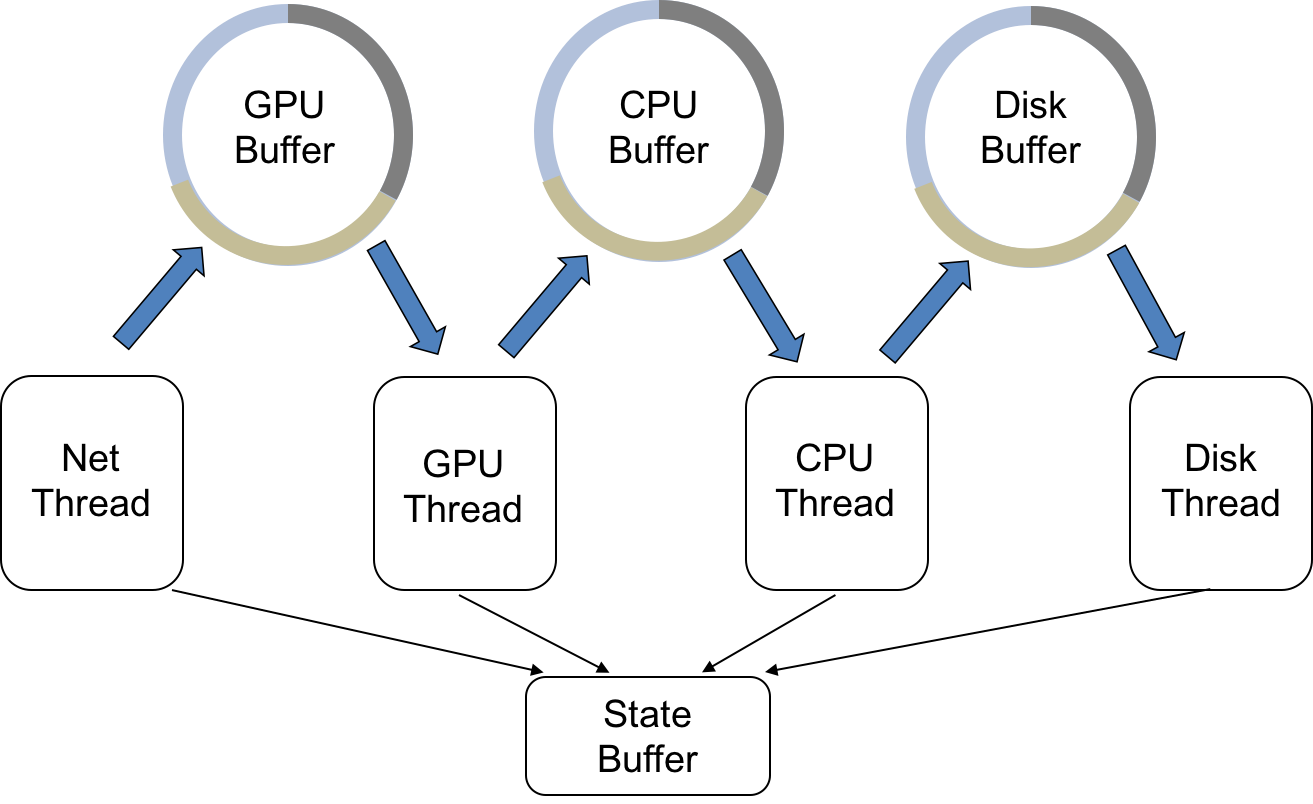
\includegraphics[width=0.7\textwidth]{./picture/hashpipe.eps}
\caption{Hashpipe thread manager structure.\label{fig:hashpipe}}
\end{figure}

\section{Local Network Framework \label{sec:Local Network}}
\subsection{Packet Format \label{sec:Data formate}}
The packet format for the system can be found in Figure \ref{fig:data_formate}. The header is 8 Bytes divided into 6 Bytes for 'Mcnt', 1 byte for 'Fid', and 1 byte for 'Xid'. 'Mcnt' is used to count the number of packets. At a given time, 'Mcnt' should the same between different ROACH2 nodes. Hashpipe will evaluate packet loss from the 'Mcnt' sequence. 'Fid' stands for F-engine ID and gives information about which ROACH2 node the packet is from. Because every GPU node has four GPU cores, each will process $\frac{1}{N_{GPU}}$ total bandwidth, where $N_{GPU}$ stands for total number of GPU cores in the system. Packets come from 4 different source IPs in one GPU node, and each node uses 'Xid' to know which GPU core the packet is going to and which frequency band the packet is from. 
\begin{figure}[t]
\centering
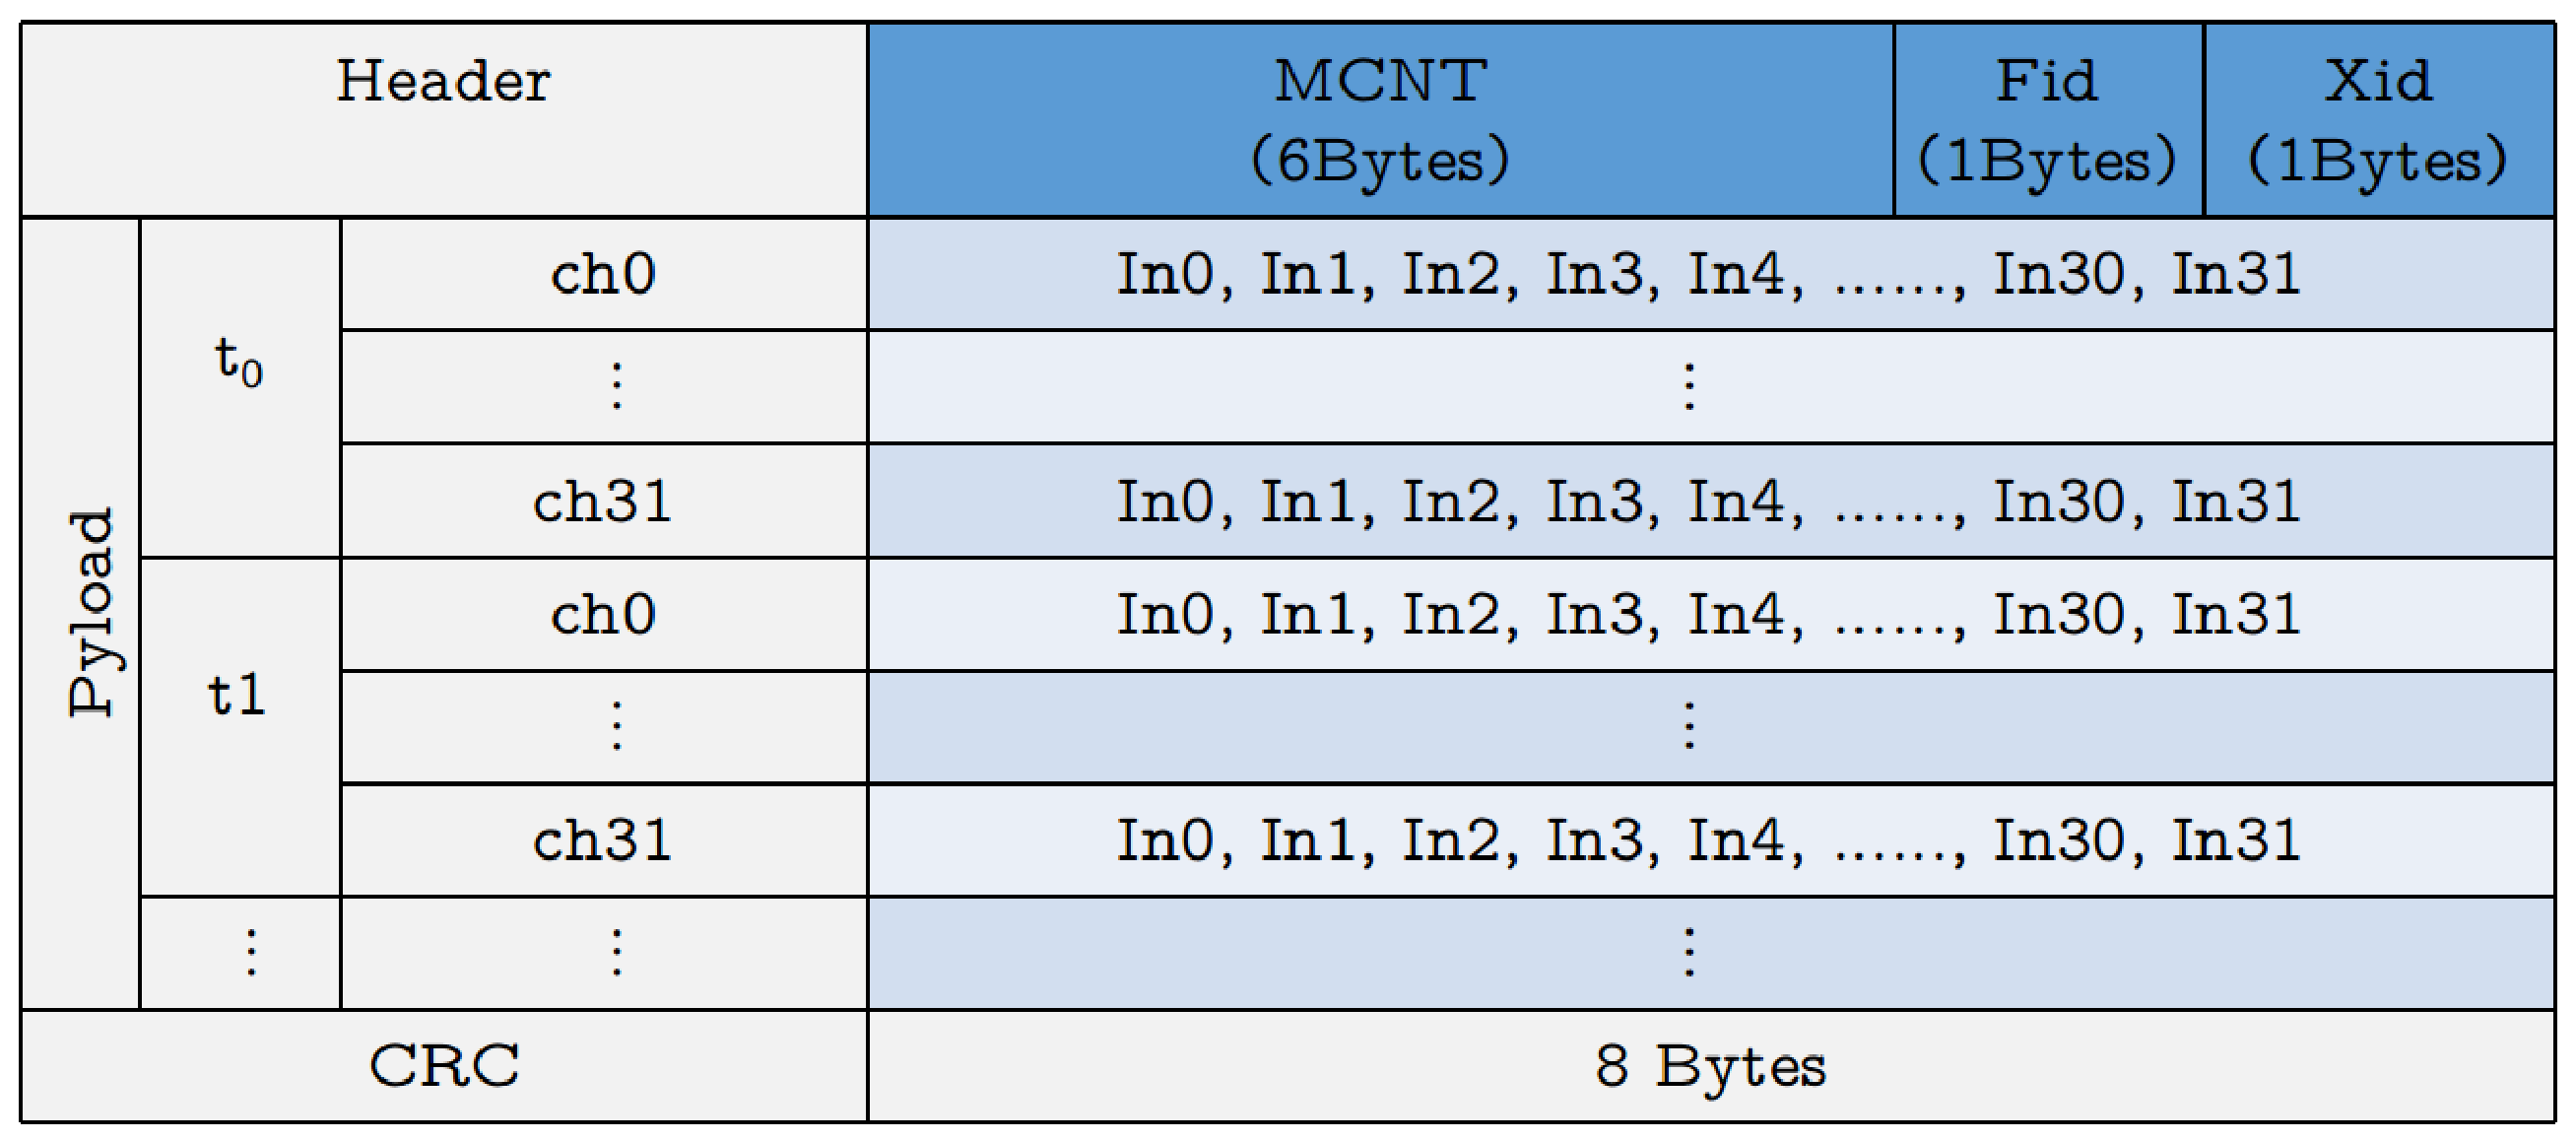
\includegraphics[width=0.9\textwidth]{./picture/Packet.eps}
\caption{Packet Data Format in our system. For 512 FFT length model ,each time is from $ch0$ to $ch15$\label{fig:data_formate}}
\end{figure}

	The payload's data shape is formatted as $[time, channel, input]$, In Figure \ref{fig:data_formate}, 'In0' means data from input 0. The data from the F-engine output is a complex number with 4 bits corresponding to a real part and 4 bits corresponding to an imaginary part. There are $\frac{1}{32}$ frequency bands equal to $\frac{1024}{32}=32$ frequency channels in each packet. In order to optimize the 10 Gbe data transfer, we add 8 time channels from the next time stamp at same frequency band to each packet. So the total size for one output packet from F-engine is:
\begin{equation} 
N_{chan}  \times N_{input} \times 8 + Header + CRC = 8208  (Bytes)
\end{equation}

\subsection{IP Assignment Strategy\label{sec:IP assignment}}
The junction between the F-engine and the X-engine is a 10 Gbe Switch. In our system, every ROACH2 node has 4 10Gbe ports, and each GPU node also has four 10 Gbe ports. As a result, we need a total of $4\times 6 $ Roach2 nodes + $4 \times 8 $ GPU nodes = 56 ports on each 10Gbe switch. To satisfy this, we use the Mellanox SX1024 Switch which has 48 ports of 10Gbe and 12 ports of 40Gbe. The 12 ports of 40 GbE can be split into $12\times4=48$ ten GbE ports.

	We denote $i \in[0,1,2,3]$ for the 10 Gbe ports on each ROACH2 node. After the transpose function model, the output from the $i$th port of ROACH2 board will contain $\frac{BW}{4} \times i $ to $\frac{BW}{4} \times (i+1)$ frequency points between 8 packets going to different GPU cores. Taking port 0 for example, we will have 0\--256 frequency points. As each GPU core processes 32 frequency points, the data output from Port 0 must be sent to 8 GPU cores. Given that each GPU node has 4 GPU cores, only two nodes are required to receive the data, namely, node0 and node1.  Thus we can put the 10Gbe switch into 4 subnets using Vlan, which will direct the data from port 0 of each ROACH2 board to GPU node0 and node1. The packet received in the GPU core will recognize the data source from the 'Fid' in Header, as introduced in section \ref{sec:Data formate}.
\begin{figure}[t]
 \centering
 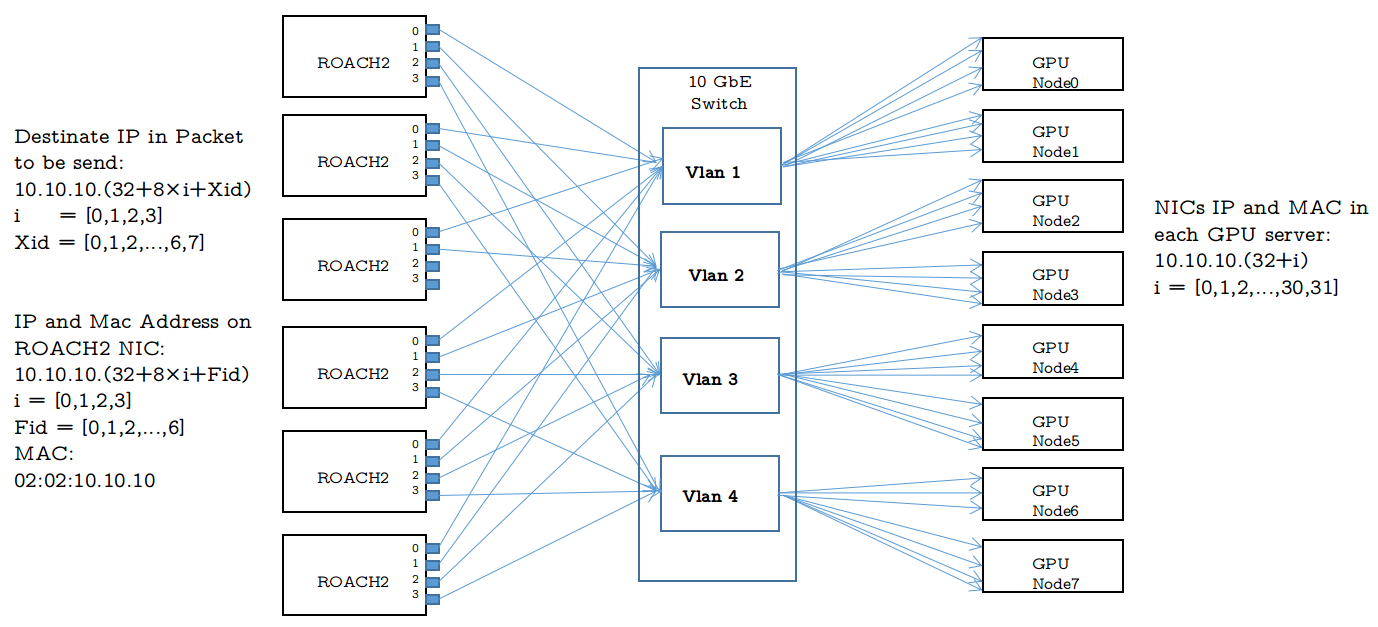
\includegraphics[width=0.9\textwidth]{./picture/Network.eps}
 \caption{Network and IP strategy in our system. We divide the 10 Gbe Switch into four Vlans to avoid packets loss}
\end{figure}

\section{Experiment}\label{sec:experiment}
We have performed several tests on this system. In our tests we had 6 ROACH2 nodes but only 1 GPU node. Thus we could only handle 1/8th of the frequency band from all inputs. 
\subsection{ADC and F-engine experiment}
We designed a ADC sampling model on the ROACH2 which packaged raw ADC samples directly and sent them to the GPU server without doing the FFT, Equalizer, Transpose etc. In the experiment, we input a 20MHz single tone analog signal into the ADC. Then, receiving data from the GPU node, we output the digitized signal and fit its frequency. The result was a sine wave with a frequency of 20.0001 MHz, which gives an error of $10^{-6}$. 

%\begin{figure}
%\epsscale{1}[ht!]
%\plottwo{adc_sample.png}{sun.png}
%\caption{Left is ADC sample experiment. The blue dot is digitalized signal , Green line is fit data with unknow phase and frequency . The fresult frequency we got has a error %$10^{-6}$. Right one is phase between two telescope from observing of sun.%\label{fig:adc}}
%\end{figure}
We also did a frequency chirp test in the F-engine. We input a single tone analog signal, and after the F-engine. We used Wireshark instead of Hashpipe in the GPU node to grab the packet from the F-engine, and found the data point in right place.
\subsection{Whole system test}
In the correlation of two inputs, phase of visibility is dependent upon the signal time delay $\tau$ between two antennas. If the input signal behaves like $Ae^{i(2\pi ft + \phi)}$, two antennas with delay $\tau$ between them will have different inputs: $Ae^{i(2\pi ft + \phi)}$ and  $Ae^{i(2\pi f(t+\tau) + \phi)}$, where $c$ is speed of light. After correlation, visibility is:
\begin{equation}
V = I_1^*\cdot I_2=Ae^{-i(2\pi ft + \phi)} \cdot Ae^{i(2\pi f(t+\tau) + \phi)} = I e^{i2\pi f\tau}
\end{equation}
The phase of visibility is $\Phi =(2\pi \tau )f$, and varies from $[-\pi, \pi]$.  When the delay $\tau$ is a constant, phase will be linear with frequency, and will have a slope of $k =2\pi \tau $. We did two experiments to simulate the effects of a time delay. In the first we generated the time delay in the FPGA design, and then added Gaussian White Noise (GWN) to the two inputs. As we knew the time delay from the FPGA design, we added $2.5\times 10^{-8}$s a time delay to our signal, giving a theoretical slope of  $k=1.571\times 10^{-7}$rad/Hz. The $k_c$ we found from correlator was $k_c = 1.561 \times 10^{-7}$ rad/Hz, which gives an error of $0.6\%$.
The other experiment we did was to put a $7.5m$ radio cable between two input signals, simulating a time delay due to distance of signal travel. We found the speed the radio signal travel through the wire is 0.7c.
\subsection{Observation Test}
We have also used this correlator to observe the Sun, Cygnus A, and other radio sources. It was able to detect the interference fringe caused by source movement. Additionally, in a collaborative observation with another correlator build by Institute of Automation, Chinese Academy of Sciences, we found our results were nearly identical. Figure \ref{fig:sun} shows the observation from sun.
\begin{figure}[t]
 \centering
 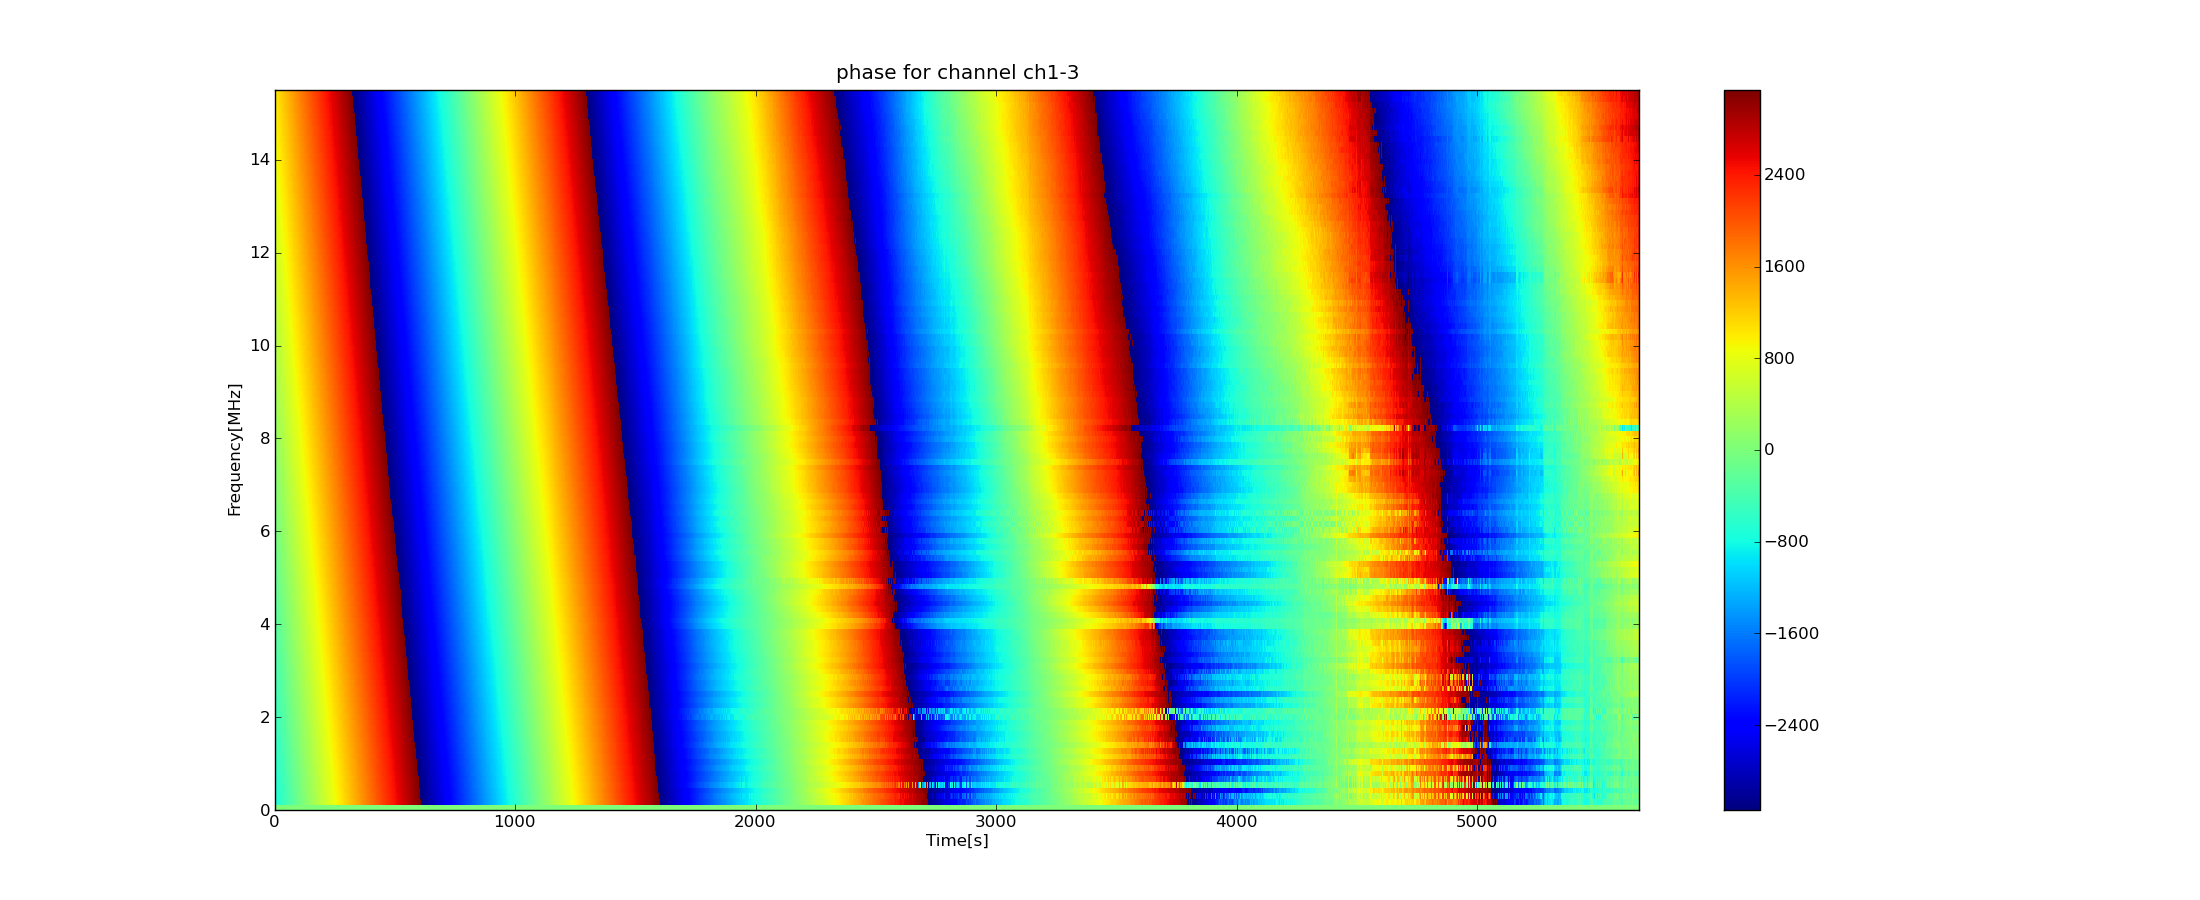
\includegraphics[width=0.9\textwidth]{./picture/sun.eps}
\caption{Phase fringe between two telescope inputs by observing of sun.\label{fig:sun}}
\end{figure}
\section{Summary}\label{sec:summary}	
The correlator system we designed based on the ROACH2-GPU framework is more flexible. We designed 1024 and 512 FFT length models for different frequency resolutions, and an ADC sampling model to store the raw data sampled by ADC. In the correlator, the F-engine gateware is the same in the different ROACH2 nodes. The computing ability of the X-engine is satisfied and we have enough 10 Gbe ports on the Switch. In the future, we can enlarge the antenna inputs simply by adding ROACH2 nodes, and will only have to change the IP and Fid configuration for each ROACH2 board. The ROACH2-SWITCH-GPU framework can also be used for different purposes at same time. Because the Switch has a broadcast mechanism, when we need to extend the spectrum data from the F-engine to another back-end like the FRB back-end, we can easily change the Switch configuration and connect the network cable to switch. Even though we developed a special model for the Tianlai Array, this system is easy to implement in other telescopes with different demands. We also did some preliminary experiments with our instrument, and the correlator system is working normally. In the future, when our whole telescope complete, the same correlator can be implemented easily. 


\bibliographystyle{ws-jai}
\bibliography{journals,Tianlai_correlator}


\end{document}